%% Overleaf
%% Software Manual and Technical Document Template
%%
%% This provides an example of a software manual created in Overleaf.

\documentclass{softwaremanual}

% Packages used in this example
\usepackage{graphicx}  % for including images
\usepackage{microtype} % for typographical enhancements
\usepackage{minted}    % for code listings
\usepackage{amsmath}   % for equations and mathematics
\setminted{style=friendly,fontsize=\small}
\usepackage[english]{babel}
\usepackage{enumitem}
\usepackage{hyperref}
\usepackage{booktabs}
\usepackage{subcaption, ragged2e}
\usepackage{chngcntr}
\counterwithin{figure}{section}
\counterwithin{table}{section}
% \usepackage[a4paper,top=4.2cm,bottom=4.2cm,left=3.5cm,right=3.5cm]{geometry} % for setting page size and margins
\usepackage[a4paper,top=2.54cm,bottom=2.54cm,left=3.17cm,right=3.17cm]{geometry} % for setting page size and margins

\usepackage{titlesec}
\setcounter{secnumdepth}{4}
\titleformat{\paragraph}
{\normalfont\normalsize\bfseries}{\theparagraph}{1em}{}
\titlespacing*{\paragraph}
{0pt}{3.25ex plus 1ex minus .2ex}{1.5ex plus .2ex}


% Custom macros used in this example document
\newcommand{\doclink}[2]{\href{#1}{#2}\footnote{\url{#1}}}
\newcommand{\cs}[1]{\texttt{\textbackslash #1}}
% \renewcommand{\listoflistingscaption}{List of Code Listings}
\def\pppx{\texttt{pppx}}
% \newcommand{\pppxversion}{1.2.1}

% Frontmatter data; appears on title page
\title{PPPx User Manual}
\version{1.3.0} % fallback version for Overleaf/local builds
\IfFileExists{version.tex}{\input{version.tex}}{}
\author{Yuanxin Pan}
\softwarelogo{
\includegraphics[width=8cm]{figs/logo}}

\begin{document}

\maketitle

\pagenumbering{roman}

\tableofcontents
\newpage

\pagenumbering{arabic}

\section{Introduction}

% This document is an example of a software manual created using \LaTeX\ and Overleaf. It provides a nice clean format for producing this type of technical document. 

% To change the logo shown on the front page, simply upload your own logo image file (via the file-tree menu) to replace the default logo.pdf file. 

% Once you're familiar with the editor, you can find various project settings in the Overleaf menu, accessed via the button in the very top left of the editor. To view tutorials, user guides, and further documentation, please visit our \doclink{https://www.overleaf.com/learn}{help library}. If you haven't used \LaTeX\ before, our \doclink{https://www.overleaf.com/learn/latex/Learn_LaTeX_in_30_minutes}{Learn \LaTeX\ in 30 minutes} tutorial is an excellent place to start.

% \subsection{Purpose of the software}


\subsection{Overview}

PPPx is a software package developed for multi-GNSS data processing. Its main component \pppx{}, dedicated to multi-GNSS positioning, is introduced in this manual. Its primary features are listed below:
\begin{enumerate}
    \item Supports four solution modes:
    \begin{enumerate}
        \item SPP: Single Point Positioning
        \item PPP: Precise Point Positioning
        \item RTK: short baseline processing
        \item TDP: Time-Differenced Positioning
    \end{enumerate}

    \item Supports multi-GNSS: GPS, GLONASS, Galileo, Beidou-2/3, and QZSS
    \item Supports multiple solvers: Extended Kalman Filter (EKF), Factor Graph Optimization (FGO), and Least-Squares Estimator (LSQ)
    \item Supports PPP-AR with Observable-specific Signal Bias (OSB) products
    \item Flexible frequency selection (L1/L2/E1/E5a/...)
    \item High precision and efficiency: capable of processing 2880 epochs within 1--2 s
    \item Unified input/output for different solution modes
    \item Supports Linux, Windows, and macOS
\end{enumerate}

% NOTE: Kinematic GNSS data collected on moving vehicles are not tested with \pppx{} yet.

% You may ask: \textbf{Why should I used \pppx{} for GNSS data processing?}

% Ans: Compared to other software, \pppx{} is easy to use, high-precision and computation efficient.

\subsection{License}

This software is distributed under the \href{https://www.gnu.org/licenses/gpl-3.0.en.html}{GPL-3.0} license.

\section{Getting started}

This section introduces the system requirements and installation steps for \pppx{}
on the supported platforms (Linux, macOS, and Windows).

%To download the latest version of \pppx{}, please have a look on \href{https://github.com/pppx-dev/pppx/releases}{this page}. Note that only the dynamically linked version of \pppx{} is provided for macOS and Windows, but a statically linked version called \texttt{pppx\_static} is additionally provided for Linux.



\subsection{System requirements}

Generally, there is no specific hardware requirement for \pppx{}.
To process a 24-hour GNSS observation file with a sampling rate of 30 s,
\pppx{} consumes around 150 MB of resident memory and one CPU core.
The resident memory consumed may, however, vary with the number of GNSS systems used
and the data sampling rate.

Note that \pppx{} only supports Macs with Apple silicon (i.e., ARM architecture)
and a macOS version newer than Monterey.



\subsection{Installation}

\subsubsection{Linux}
\label{sec:installation_linux}

This application is distributed as an \href{https://appimage.org/}{AppImage},
making it portable across most modern Linux distributions.
Specifically, \pppx{} is built on Ubuntu 20.04 and requires the host system
to have GNU C Library (\texttt{glibc}) version 2.31 or newer.

It is compatible with the following distributions (and any of their derivatives):

\begin{table}[h]
\centering
\renewcommand{\arraystretch}{1.25}
\begin{tabular}{p{0.35\textwidth} p{0.55\textwidth}}
    \hline
    Distribution Family & Supported Versions \\ 
    \hline
    Ubuntu & 20.04 LTS, 22.04 LTS, 24.04 LTS (and newer) \\ 
    Linux Mint & 20, 21, 22 (and newer) \\ 
    Debian & 11 ``Bullseye'', 12 ``Bookworm'' (and newer) \\ 
    Fedora & 32 (and newer) \\ 
    RHEL / Rocky / Alma & 9.x (and newer) \newline \textit{Note: RHEL 8 is not supported} \\ 
    openSUSE & Leap 15.3+, Tumbleweed \\ 
    Arch Linux / Manjaro & Rolling releases (Always updated) \\ 
    \hline
\end{tabular}
\end{table}

\vspace{1em}
\textit{\textbf{Not sure if your system is supported?}}

You can easily check your system's \texttt{glibc} version
by running the \texttt{ldd --version} command in your terminal.


Clone the repository and run the installer from its root folder:

\begin{minted}[frame=leftline]{bash}
git clone --depth 1 https://github.com/pppx-dev/pppx.git
cd pppx
./install.sh
\end{minted}

The installer downloads the latest \pppx{} executable, installs both \pppx{} and the
wrapper script \texttt{pppx.sh} to \verb|~/.local/bin|, and configures \texttt{pppx.sh}
to use the \texttt{table} files in the cloned repository. Keeping the repository is
recommended, as it provides the \texttt{table} files and examples used by \pppx{}.



\subsubsection{Windows}
\label{sec:installation_windows}

The easiest way to run \pppx{} on Windows is to use the Windows Subsystem for Linux (WSL);
simply follow the instructions in Section~\ref{sec:installation_linux}.
However, \pppx{} can also run natively on Windows
using PowerShell or Command Prompt (\texttt{cmd.exe}).


Clone the repository, then run the installer from its root folder in PowerShell.
It will download the executable, fetch the required DLLs, and add the software
(\path{C:\Users\<YOUR_USER_NAME>\AppData\Local\Programs\PPPx}) to your user \texttt{PATH}:

\begin{minted}[frame=leftline]{powershell}
git clone --depth 1 https://github.com/pppx-dev/pppx.git
cd pppx
.\install.ps1
\end{minted}

\textbf{Note}: You must restart PowerShell, cmd.exe, or Git Bash after the installation.

The installer also installs and configures the wrapper script \texttt{pppx.sh}
(pointing it at the \texttt{table} folder in the cloned repository). While \texttt{pppx.sh}
cannot run in PowerShell or \texttt{cmd.exe}, you can run it from \textbf{Git Bash}, which
is bundled with \href{https://git-scm.com/download/win}{Git for Windows} (the same tool
used for \texttt{git clone}). Product downloads rely on \texttt{curl}, which Git Bash
provides:

\begin{minted}[frame=leftline]{bash}
# In Git Bash
pppx.sh -c pppx.ini rinex/ZIM200CHE_R_20221000000_01D_30S_MO.rnx
\end{minted}


% \paragraph{With MSYS2}

% It is recommended to use \pppx{} on Windows 10 or higher.

% % For Windows 7 or 8 users, please refer to \href{https://www.msys2.org/docs/windows_support/}{this page} to install a old version of \texttt{MSYS2} for software installation.

% If you don't have \texttt{MSYS2} installed on your PC yet, please install it according to \href{https://www.msys2.org}{this page}.

% Then, open \texttt{MSYS2 MINGW64} and run the following comands:
% \begin{minted}[frame=leftline]{bash}
%   $ pacman -Syu   # update package library
%   $ pacman -S git mingw-w64-x86_64-ceres-solver

%   $ git clone git@github.com:pppx-dev/pppx.git
%   $ mkdir -p ${HOME}/.local/bin/
%   $ cp pppx.exe ${HOME}/.local/bin/
% \end{minted}



\subsubsection{macOS}
\label{sec:installation_macos}

\pppx{} only supports Macs with Apple silicon and a macOS version newer than Monterey.


\paragraph{Prerequisite}

If you do not have \href{https://brew.sh/}{Homebrew} on your Mac, please install it first:

\begin{minted}[breaklines, frame=leftline]{bash}
  $ /bin/bash -c "$(curl -fsSL https://raw.githubusercontent.com/Homebrew/install/HEAD/install.sh)"
\end{minted} 

\pppx{} is linked against the latest \texttt{ceres-solver} library, so make sure you have the
latest version installed as well in order to run \pppx{} properly on your Mac.
Run the following command in the Terminal application:

\begin{minted}[frame=leftline]{bash}
brew install ceres-solver
\end{minted}


Clone the repository and run the installer from its root folder in the Terminal:

\begin{minted}[frame=leftline]{bash}
git clone --depth 1 https://github.com/pppx-dev/pppx.git
cd pppx
./install.sh
\end{minted}

The installer downloads the latest \pppx{} executable, bypasses Apple's quarantine
security check, installs both \pppx{} and the wrapper script \texttt{pppx.sh} to
\verb|~/.local/bin|, and configures \texttt{pppx.sh} to use the \texttt{table} files in
the cloned repository. Keeping the repository is recommended, as it provides the
\texttt{table} files and examples used by \pppx{}.


\section{Usage}
\label{sec:usage}

This section introduces how to use the \pppx{} software. The general steps to run \pppx{} are:
\begin{enumerate}
    \item Prepare input files, including a GNSS observation file in the Receiver Independent
          Exchange (RINEX) format and necessary products
          (either broadcast ephemeris or precise products from IGS)
    \item Modify the configuration file \textit{pppx.ini} if necessary
    \item Execute \pppx{} from the command line: \newline
    \texttt{pppx -c pppx.ini path-to-rnxobs [rnxobs-of-base]}
    \item Check output files
\end{enumerate}

Here are some example commands to run \pppx{}:
\begin{minted}[breaklines, frame=leftline]{bash}
  # SPP/PPP/TDP
  # (Note: TDP is suitable for high-frequency data, e.g., 1 Hz)
  $ pppx -c pppx.ini rinex/ZIM200CHE_R_20221000000_01D_30S_MO.rnx

  # RTK
  # (ZIMM is the base station in this example)
  $ pppx -c pppx.ini rinex/ZIM200CHE_R_20221000000_01D_30S_MO.rnx rinex/ZIMM00CHE_R_20221000000_01D_30S_MO.rnx
\end{minted}

To make GNSS data processing easier, a wrapper script (scripts/pppx.sh) is provided that
automatically downloads the necessary products (e.g., SP3, CLK, OBX, BIA, ERP, BRDC, and GIM)
from the \href{ftp://ftp.aiub.unibe.ch/CODE}{CODE} FTP server and then invokes \pppx{}.
The recommended steps to use this wrapper script are:
\begin{minted}[breaklines, frame=leftline]{bash}
  $ pppx -x ppp > pppx.ini  # generate a default config file

  # Then, edit pppx.ini if necessary but keep [product] (except "src") and [table] blank
  $ pppx.sh -c pppx.ini rinex/ZIM200CHE_R_20221000000_01D_30S_MO.rnx
\end{minted}

\textbf{NOTE}: \texttt{pppx.sh} is installed and configured automatically by the installer
(\texttt{install.sh} on Linux/macOS, \texttt{install.ps1} on Windows), pointing it at the
\texttt{table} folder in your cloned repository, so \texttt{pppx.sh -c ...} works out of the
box. It runs natively on Linux and macOS, and on Windows via Git Bash. It requires only
\texttt{curl} and standard Unix tools (no \texttt{wget} needed), which are available by
default on these platforms.



\subsection{Input}
\label{sec:input}

The complete list of input files is provided below:
\begin{itemize}
    \item GNSS observations in the RINEX format, specified by command line arguments
    \item Configuration file \texttt{pppx.ini}, specified by command line argument
    \item Satellite products (either brdc or precise), specified by \texttt{pppx.ini}
    \item Table files (already provided in the table/ directory), specified by \texttt{pppx.ini}
\end{itemize}

The configuration file and satellite products will be explained in detail in subsequent sections.



\subsubsection{Configuration}
\label{sec:input_configuration}

The configuration file \texttt{pppx.ini} is the primary interface to \pppx{}.
Written in the human-readable \texttt{ini} format, it lets users specify the GNSS positioning
strategy through the sections listed in Table~\ref{tab:config}.

\begin{table}[!hbt]
    \centering
    \caption{Available sections of the configuration file \texttt{pppx.ini}.}
    \label{tab:config}
    \resizebox{\textwidth}{!}{
    \begin{tabular}{p{0.18\linewidth}  p{0.85\linewidth}}
    \toprule
        Section & Description \\
    \midrule
        session & The desired sampling rate and start and end time for data processing \\
        constellation & The GNSS systems to be used and specific satellites to be excluded \\
        observation & Selection of signal frequency and observable priority \\
        model & The tropospheric and ionospheric models \\
        estimation & Various estimation strategies, including solution mode, positioning mode, solver type, etc. \\
        product & The choice of satellite product source and the path to each product \\
        table & The paths to table files \\
        output & The output path and log level \\
    \bottomrule
    \end{tabular}}
\end{table}

Some example configuration files are provided in the folder "example/pppx/".
Most settings in \texttt{pppx.ini} are self-explanatory.
Usually, users just need to modify the following settings
and leave the rest at their default values:

\begin{minted}[frame=leftline]{ini}
[constellation]: system
[estimation]: sol_mode, pos_mode, solver
[product]: src, nav, sp3, clk
\end{minted}

If no template configuration file is available, you can generate a default configuration for a
specific solution mode (spp, ppp, rtk, or tdp) with the command below.
Redirect its output to a file to obtain a ready-to-edit configuration
for processing data with \pppx{}.

\begin{minted}[frame=leftline]{bash}
  # Output the default configurations for SPP and redirect them to a file
  $ pppx -x spp > spp.ini
\end{minted}

% Although most settings are shared by different sol\_mode (i.e., spp/ppp/rtk/tdp), some settings are sol\_mode specific:

% \begin{minted}[frame=leftline]{ini}
% [model]: trop, iono
% ; Currenty, they are not effective for rtk
% ; Tropospheric and ionospheric delays are ignored for short baselines
% ; iono can only be IF for ppp

% [estimation]: solver
% ; spp/tdp: only lsq and fgo are supported
% ; ppp: only ekf and fgo are supported
% ; rtk: only ekf is supported

% [estimation]: slip_det
% ; only effective for ppp
% ; rtk and tdp always use LLI and GF to detect cycle slips

% [estimation]: pos_pri, clk_pri, isb_pri, ztd_pri
% ; only effective for KF-based PPP
% ; ztd_pri is also valid for FGO-based PPP
% \end{minted}

The following paragraphs explain how to set the key--value pairs in each section of the
configuration file.


\paragraph{session}

Here, \underline{"interval"} specifies the processing interval; it must be no smaller than the
sampling rate of the RINEX file and an integer multiple of it.
\underline{"date"} denotes the year and day of year (DOY) for data processing
and is used to replace the placeholders in the "[product]" section.
If left blank, it is read from the first epoch of the RINEX file.
\underline{"start"} and \underline{"end"} denote the start and end epochs for data processing
within the day (closed interval).

Figure~\ref{fig:conf_session} shows example settings.
In most cases, all fields in this section can be left blank,
and \pppx{} will then process the entire RINEX file epoch by epoch.

\begin{figure}[!hbt]
    \centering
    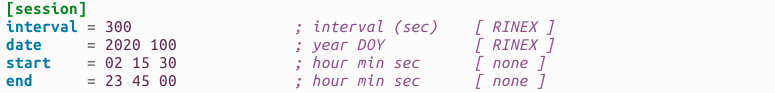
\includegraphics[width=1.1\linewidth]{figs/usage/conf_session.png}
    \caption{The "session" section of configuration.}
    \label{fig:conf_session}
    \vspace{-8pt}
\end{figure}


\paragraph{constellation}

This section defines the GNSS systems to be used for data processing
and the problematic satellites to be excluded.
An example is shown in Figure~\ref{fig:conf_constellation}.
Note that the order of the letters (e.g., GRECJ) does not matter,
and there must be no spaces between them.
The GPS system is not mandatory; Galileo-only solutions, for example, are also feasible.
The excluded PRNs should be separated by whitespace.

\begin{figure}[!hbt]
    \centering
    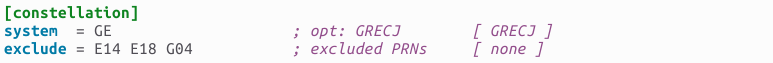
\includegraphics[width=1.1\linewidth]{figs/usage/conf_constellation.png}
    \caption{The "constellation" section of configuration.}
    \label{fig:conf_constellation}
    \vspace{-8pt}
\end{figure}


\paragraph{observation}
This section is documented thoroughly by the comments in the configuration file.
Note that the observation noise represents the noise level of the uncombined observations;
for ionosphere-free combinations, the observation noise is computed automatically
from the uncombined values.
A screenshot of the example settings is provided in Figure~\ref{fig:conf_observation}.

\begin{figure}[!hbt]
    \centering
    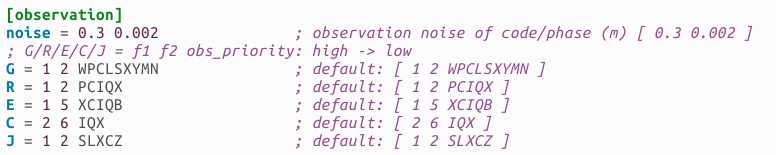
\includegraphics[width=1.1\linewidth]{figs/usage/conf_observation.png}
    \caption{The "observation" section of configuration.}
    \label{fig:conf_observation}
    \vspace{-8pt}
\end{figure}


\paragraph{model}
This section specifies the tropospheric and ionospheric models.
An example is provided in Figure~\ref{fig:conf_model}.
Users should choose an option (case sensitive) from the values listed in the comments.
Note that this section has no effect for RTK,
since tropospheric and ionospheric delays are ignored for short baselines;
"iono" can only be IF for PPP.

Currently, the tide model cannot be configured through \texttt{pppx.ini}.
Solid Earth tide, ocean tidal loading, and pole tide are applied for PPP whenever possible,
but not for spp/rtk/tdp.

\begin{figure}[!hbt]
    \centering
    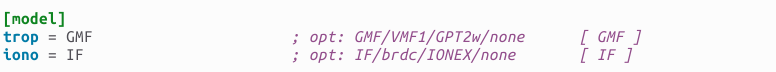
\includegraphics[width=1.1\linewidth]{figs/usage/conf_model.png}
    \caption{The "model" section of configuration.}
    \label{fig:conf_model}
    \vspace{-8pt}
\end{figure}


\paragraph{estimation}

This is the most important section of the configuration file.
Here, you can choose the solution mode (spp/ppp/rtk/tdp),
positioning mode (kinematic/static/fixed), and solver (ekf/fgo/lsq) used for adjustment.
An example is provided in Figure~\ref{fig:conf_estimation}.
Most settings are self-explanatory.

The fields \underline{"sol\_mode"}, \underline{"pos\_mode"}, and \underline{"solver"}
are well explained in the configuration file.
Note, however, that spp and tdp support only the kinematic positioning mode,
and not every solver is supported for each solution mode
(lsq and fgo for spp and tdp; ekf and fgo for ppp and rtk).
The software will output an error message if a given configuration is not supported.

\underline{"fgo\_var"} controls the output of variance information
when fgo is specified as the "solver".
By default, variances are not computed for fgo, because doing so can be time-consuming.

\underline{"site\_pos"} specifies the approximate station coordinates in XYZ format (unit: meters).
If not specified, the approximate coordinates are computed automatically using SPP.
The same rule applies to the field \underline{"base\_pos"} for rtk.

\underline{"ppp\_ar"} is a switch for PPP-AR.
Ambiguity resolution is enabled by setting it to "yes", in which case a valid phase-bias product
must be provided through the field "[product] bia".
The LAMBDA and rounding methods are used to resolve integer ambiguities
when "solver" is set to "ekf" and "fgo", respectively.
Note that GLONASS is disabled for AR
and that the GPS L5 signal is currently not supported for PPP-AR.

\underline{"sf\_ppp"} is designed to run single-frequency PPP with GIM products;
that is, ionospheric delays are not estimated but fixed to GIM corrections.
This makes it possible to evaluate the accuracy of GIM products.
Note that dual-frequency observations are still required for cycle slip detection,
and "ppp\_ar" should be set to "no" when sf\_ppp is enabled.

\underline{"slip\_det"} specifies the methods used for cycle slip detection in ppp.
The option "TDCP" stands for time-differenced carrier phase.
You can set "slip\_det" to "ALL" for most stations,
but "MW" should not be used for stations with noisy pseudorange, such as smartphones.
"LLI" can be unreliable, because some stations set many incorrect LLI flags,
yet it is recommended for processing smartphone GNSS data.
Note that rtk and tdp always use LLI and GF for cycle slip detection,
which is currently not configurable.

\underline{"pos\_pri"}, \underline{"clk\_pri"}, \underline{"isb\_pri"},
and \underline{"ztd\_pri"} specify the a priori uncertainties and process noises
of the station position, receiver clock, receiver inter-system bias (ISB),
and tropospheric delay for EKF, respectively.
Note that EKF estimates receiver clocks for one reference GNSS system
and estimates ISBs for other systems.
When FGO is chosen as the solver, only "pos\_pri" and "ztd\_pri" are effective
and the other "pri" settings are not used:
an individual receiver clock error (instead of an ISB) is estimated
as white noise for each constellation.

\underline{"rtk\_ar"} is a switch for RTK-AR, with "yes" as its default value.
The LAMBDA and rounding methods are used to resolve integer double-differenced (DD) ambiguities
when "solver" is set to "ekf" and "fgo", respectively.
\underline{"glonass\_ar"} can be set to "yes" for rtk
if the rover and base stations share the same receiver type; otherwise, keep it as "no".

\begin{figure}[!hbt]
    \centering
    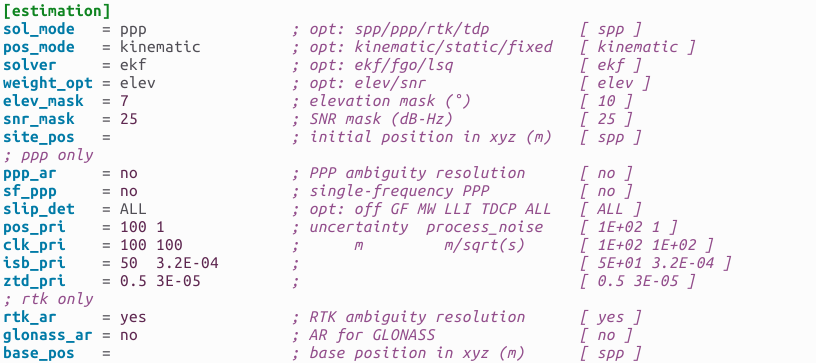
\includegraphics[width=1.15\linewidth]{figs/usage/conf_estimation.png}
    \caption{The "estimation" section of configuration.}
    \label{fig:conf_estimation}
    \vspace{-8pt}
\end{figure}


\paragraph{product}

This section specifies the paths to the various products.
If "src = brdc", then "nav" must be set to a valid path to a broadcast ephemeris.
If "src = precise", then "sp3" must be set to a valid path to an SP3 product,
and all other products are optional.
Relative paths are resolved relative to the directory where \pppx{} is executed,
not where pppx.ini is located.
In addition, placeholders (see Figure~\ref{fig:conf_product}) can be used in product names,
making it easier to process GNSS data over multiple days.
More details on the products are given in Section~\ref{sec:input_product}.

\begin{figure}[!hbt]
    \centering
    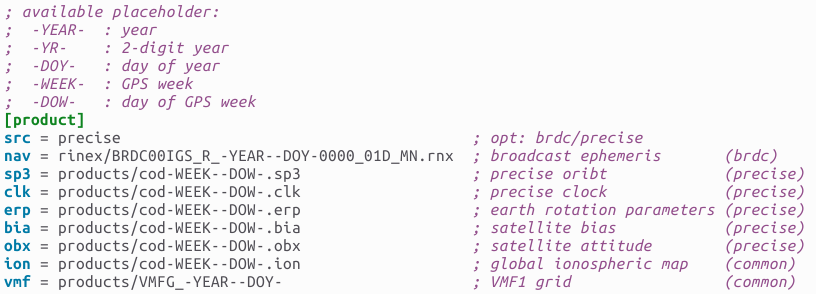
\includegraphics[width=1.15\linewidth]{figs/usage/conf_product.png}
    \caption{The "product" section of configuration.}
    \label{fig:conf_product}
    \vspace{-8pt}
\end{figure}


\paragraph{table}
This section specifies the paths to the table files.
An example is provided in Figure~\ref{fig:conf_table}.
More details can be found in Section~\ref{sec:input_table}.
As with products, relative paths are resolved relative to the directory where \pppx{} is executed.

\begin{figure}[!hbt]
    \centering
    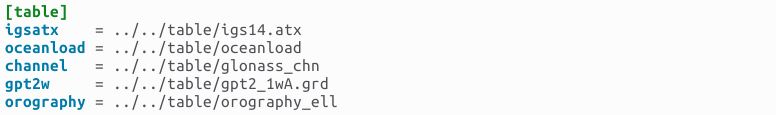
\includegraphics[width=1.15\linewidth]{figs/usage/conf_table.png}
    \caption{The "table" section of configuration.}
    \label{fig:conf_table}
    \vspace{-8pt}
\end{figure}


\paragraph{output}
This section specifies the output path and log level.
An example is provided in Figure~\ref{fig:conf_output}.
More details can be found in Section~\ref{sec:output}.

\begin{figure}[!hbt]
    \centering
    
\includegraphics[width=1.15\linewidth]{figs/usage/conf_output.png}
    \caption{The "output" section of configuration.}
    \label{fig:conf_output}
    \vspace{-8pt}
\end{figure}



\subsubsection{Product}
\label{sec:input_product}

There are two options for satellite products in each solution mode, "brdc" and "precise",
controlled by the configuration field "[product] src".
The "brdc" option uses satellite orbits and clocks computed from broadcast ephemeris,
whereas the "precise" option uses orbits and clocks from IGS precise products.
Note that "[table] igsatx" is required when "[product] src" is set to "precise".

Here are some clarifications:

\begin{itemize}[]
    \item All products labeled "precise" will not be used if "[product] src" is set to "brdc"
    \item Precise orbits and clocks can be used for SPP, but the Differential Code Bias (DCB)
          issue is not handled for single-frequency SPP; in this case, it is recommended to set
          "[model] iono = IF"
    \item Only the SP3 file is required for the "precise" option; other precise products are
          optional. If the CLK product is missing, the clock corrections from the SP3 file are used
    \item "ion" and "vmf" are only mandatory when the corresponding models are specified
    \item PPP specific:
    \begin{itemize}[noitemsep]
        \item Broadcast ephemeris can also be used for PPP;
              precise products are not used in this case
        \item The nominal attitude is used if the OBX product is missing
        \item The BIA product is used if "[estimation] ppp\_ar" is set to "yes"
        \item Pole tide corrections are not applied if the ERP product is missing,
              but this is fine for most applications
    \end{itemize}
\end{itemize}



\subsubsection{Table}
\label{sec:input_table}

Several table files are required when specific models are used for data processing.
These mainly include the antenna model, the tropospheric model, and the tide model.
A complete list of the required table files is provided in Table~\ref{tab:table}.
The instructions for downloading each table file are provided in Appendix~\ref{app:table}.

\begin{table}[!hbt]
    \centering
    \caption{List of table files.}
    \label{tab:table}
    \begin{tabular}{ll}
    \toprule
        Table & Description \\
    \midrule
        channel & Frequency channel numbers for GLONASS satellites \\
        gpt2w & Coefficients of the GPT2w tropospheric model \\
        igsatx & Satellite and receiver antenna models in the IGS ANTEX format \\
        oceanload & Ocean tide loading coefficients for stations \\
        orography & Ellipsoidal station heights of the VMF1 grid points \\
    \bottomrule
    \end{tabular}
\end{table}

Some clarifications are provided below:

\begin{itemize}[]
    \item "channel" is only needed when GLONASS carrier phase measurements are used for data
          processing (i.e., ppp/rtk/tdp)
    \item "gpt2w" must be set when "[model] trop" is set to "GPT2w"
    \item "igsatx" is mandatory if "[product] src" is set to "precise".
          When "igsatx" is specified, the satellite and station PCO corrections are applied for
          all solution modes, but the satellite and station PCV corrections are applied only for
          PPP and RTK.
    \item "oceanload" is optional; ocean tide loading is not corrected
          if the coefficients for the processed station are missing
    \item "orography" is needed when "[model] trop" is set to "VMF1"
\end{itemize}

Although table files are not always required, it is recommended to properly set all table paths
to simplify the process and avoid potential issues.



\subsection{Output}
\label{sec:output}

This section introduces the output files generated by the \pppx{} software.
An overview of these files is provided in Table~\ref{tab:output}.
The function and format of each file are described in detail in the following sections.

\begin{table}[!hbt]
    \centering
    \caption{List of output files.}
    \label{tab:output}
    \begin{tabular}{p{0.15\linewidth}  p{0.8\linewidth}}
    \toprule
        Output & Description \\
    \midrule
    pos file & Receiver position, clock (GPS) and ZTD estimates for each epoch \\
    log file & Information for debugging, including cycle slip detection, a priori and post-fit residuals, and ambiguity resolution \\
    stat file & Post-fit residuals and various estimates in the RTKLIB stat format, intended for visualization with RTKLIB \\
    \bottomrule
    \end{tabular}
\end{table}



\subsubsection{pos file}
\label{sec:output_pos}

The primary output of \pppx{} is the pos file,
which contains the main estimates for each processed epoch.
These include station coordinates in the Earth-centered and Earth-fixed (ECEF) coordinate system,
standard deviations of the coordinate estimates, receiver clock errors for the GPS system,
and Zenith Total Delays (ZTD).

Figure~\ref{fig:output_pos} shows the beginning of a sample pos file.
The units used for coordinates, clock errors, and ZTD estimates are meters.
Note that the coordinate system aligns with the satellite orbit products used for data processing.
By default, the standard deviations of coordinates are not included in the output
when "fgo" is selected as the solver, because of the long computation time required.

\begin{figure}[!hbt]
    \centering
    \hspace*{-1.2in}
    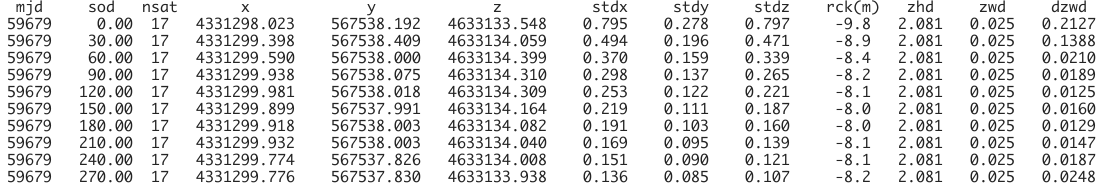
\includegraphics[width=0.95\paperwidth]{figs/usage/output_pos.png}
    \caption{The screenshot of a sample pos file.}
    \label{fig:output_pos}
    \vspace{-8pt}
\end{figure}



\subsubsection{log file}
\label{sec:output_log}

A log file will be generated if the "[output] level" in the configuration file is not set to "off".
This file contains debugging information such as cycle slip detection, outlier detection,
and a-prior and post-fit residuals.
Each log message generally begins with a letter that indicates the message type:
'T' for Trace, 'D' for Debug, 'I' for Information, 'W' for Warning,
'E' for Error, and 'C' for Critical.

Figure~\ref{fig:output_log} shows the screenshot of a sample log file.
For example, a cycle slip was detected at epoch 86370.0 (seconds of the day).
Following the PRN number, the azimuth, elevation, and between-epoch difference
of the geometry-free (GF) combination of the satellite are provided.
The subsequent line indicates that a new ambiguity parameter (numbered 410)
was introduced at that epoch.
The following lines provide information for all satellites available at that epoch.
For each satellite, listed after its PRN and epoch time, these include the a priori residuals
of pseudorange and carrier phase, the corresponding post-fit residuals,
the ambiguity estimate in cycles, and the azimuth and elevation.

\begin{figure}[!hbt]
    \centering
    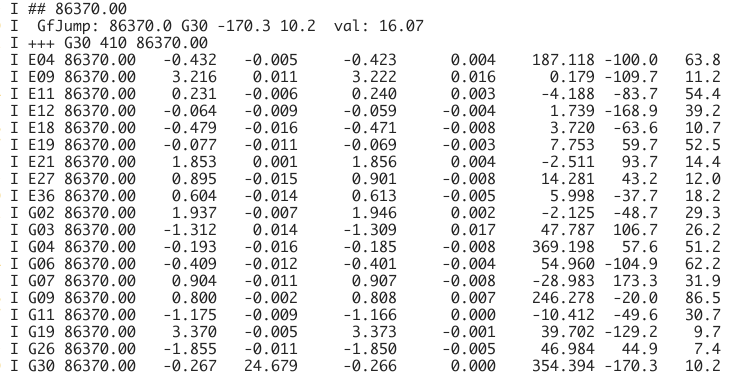
\includegraphics[width=1.0\linewidth]{figs/usage/output_log.png}
    \caption{The screenshot of a sample log file.}
    \label{fig:output_log}
    \vspace{-8pt}
\end{figure}



\subsubsection{stat file}
\label{sec:output_stat}

A stat file is always generated for visualization with the
\href{https://github.com/tomojitakasu/RTKLIB_bin/tree/rtklib_2.4.3}{RTKLIB} software.
For detailed information on the format, you can refer to the RTKLIB
\href{https://github.com/tomojitakasu/RTKLIB/blob/rtklib_2.4.3/src/rtkpos.c#L107}{source code}.
Currently, \pppx{} only outputs messages with the keywords "\$POS", "\$CLK", and "\$SAT".
The only difference is that the "\$CLK" values are expressed in meters (instead of nanoseconds)
and represent absolute clock errors for each GNSS system (rather than inter-system biases).
Figure~\ref{fig:output_stat} shows a screenshot of a sample stat file.

\begin{figure}[!hbt]
    \centering
    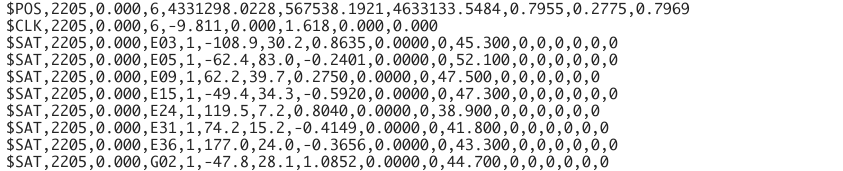
\includegraphics[width=1.2\linewidth]{figs/usage/output_stat.png}
    \caption{The screenshot of a sample stat file.}
    \label{fig:output_stat}
    \vspace{-8pt}
\end{figure}



\subsection{Visualization}
\label{sec:visualization}

This section explains how to visualize the solutions generated by \pppx{}.



\subsubsection{With the PPPx Web Viewer}
\label{sec:visualization_web}

The \href{https://app.pppx.dev}{PPPx Web Viewer} is a browser-based app for the
interactive viewing of \pppx{} results.
It accepts the \pppx{} pos and stat files as input and offers two main views:
a position time series and a map view of the solution.
Being entirely browser-based, it requires no installation and runs on any platform.
To use it, simply open \href{https://app.pppx.dev}{https://app.pppx.dev}
and load a pos or stat file.
An example is shown in Figure~\ref{fig:visualization_web}.

\begin{figure}[!hbt]
    \centering
    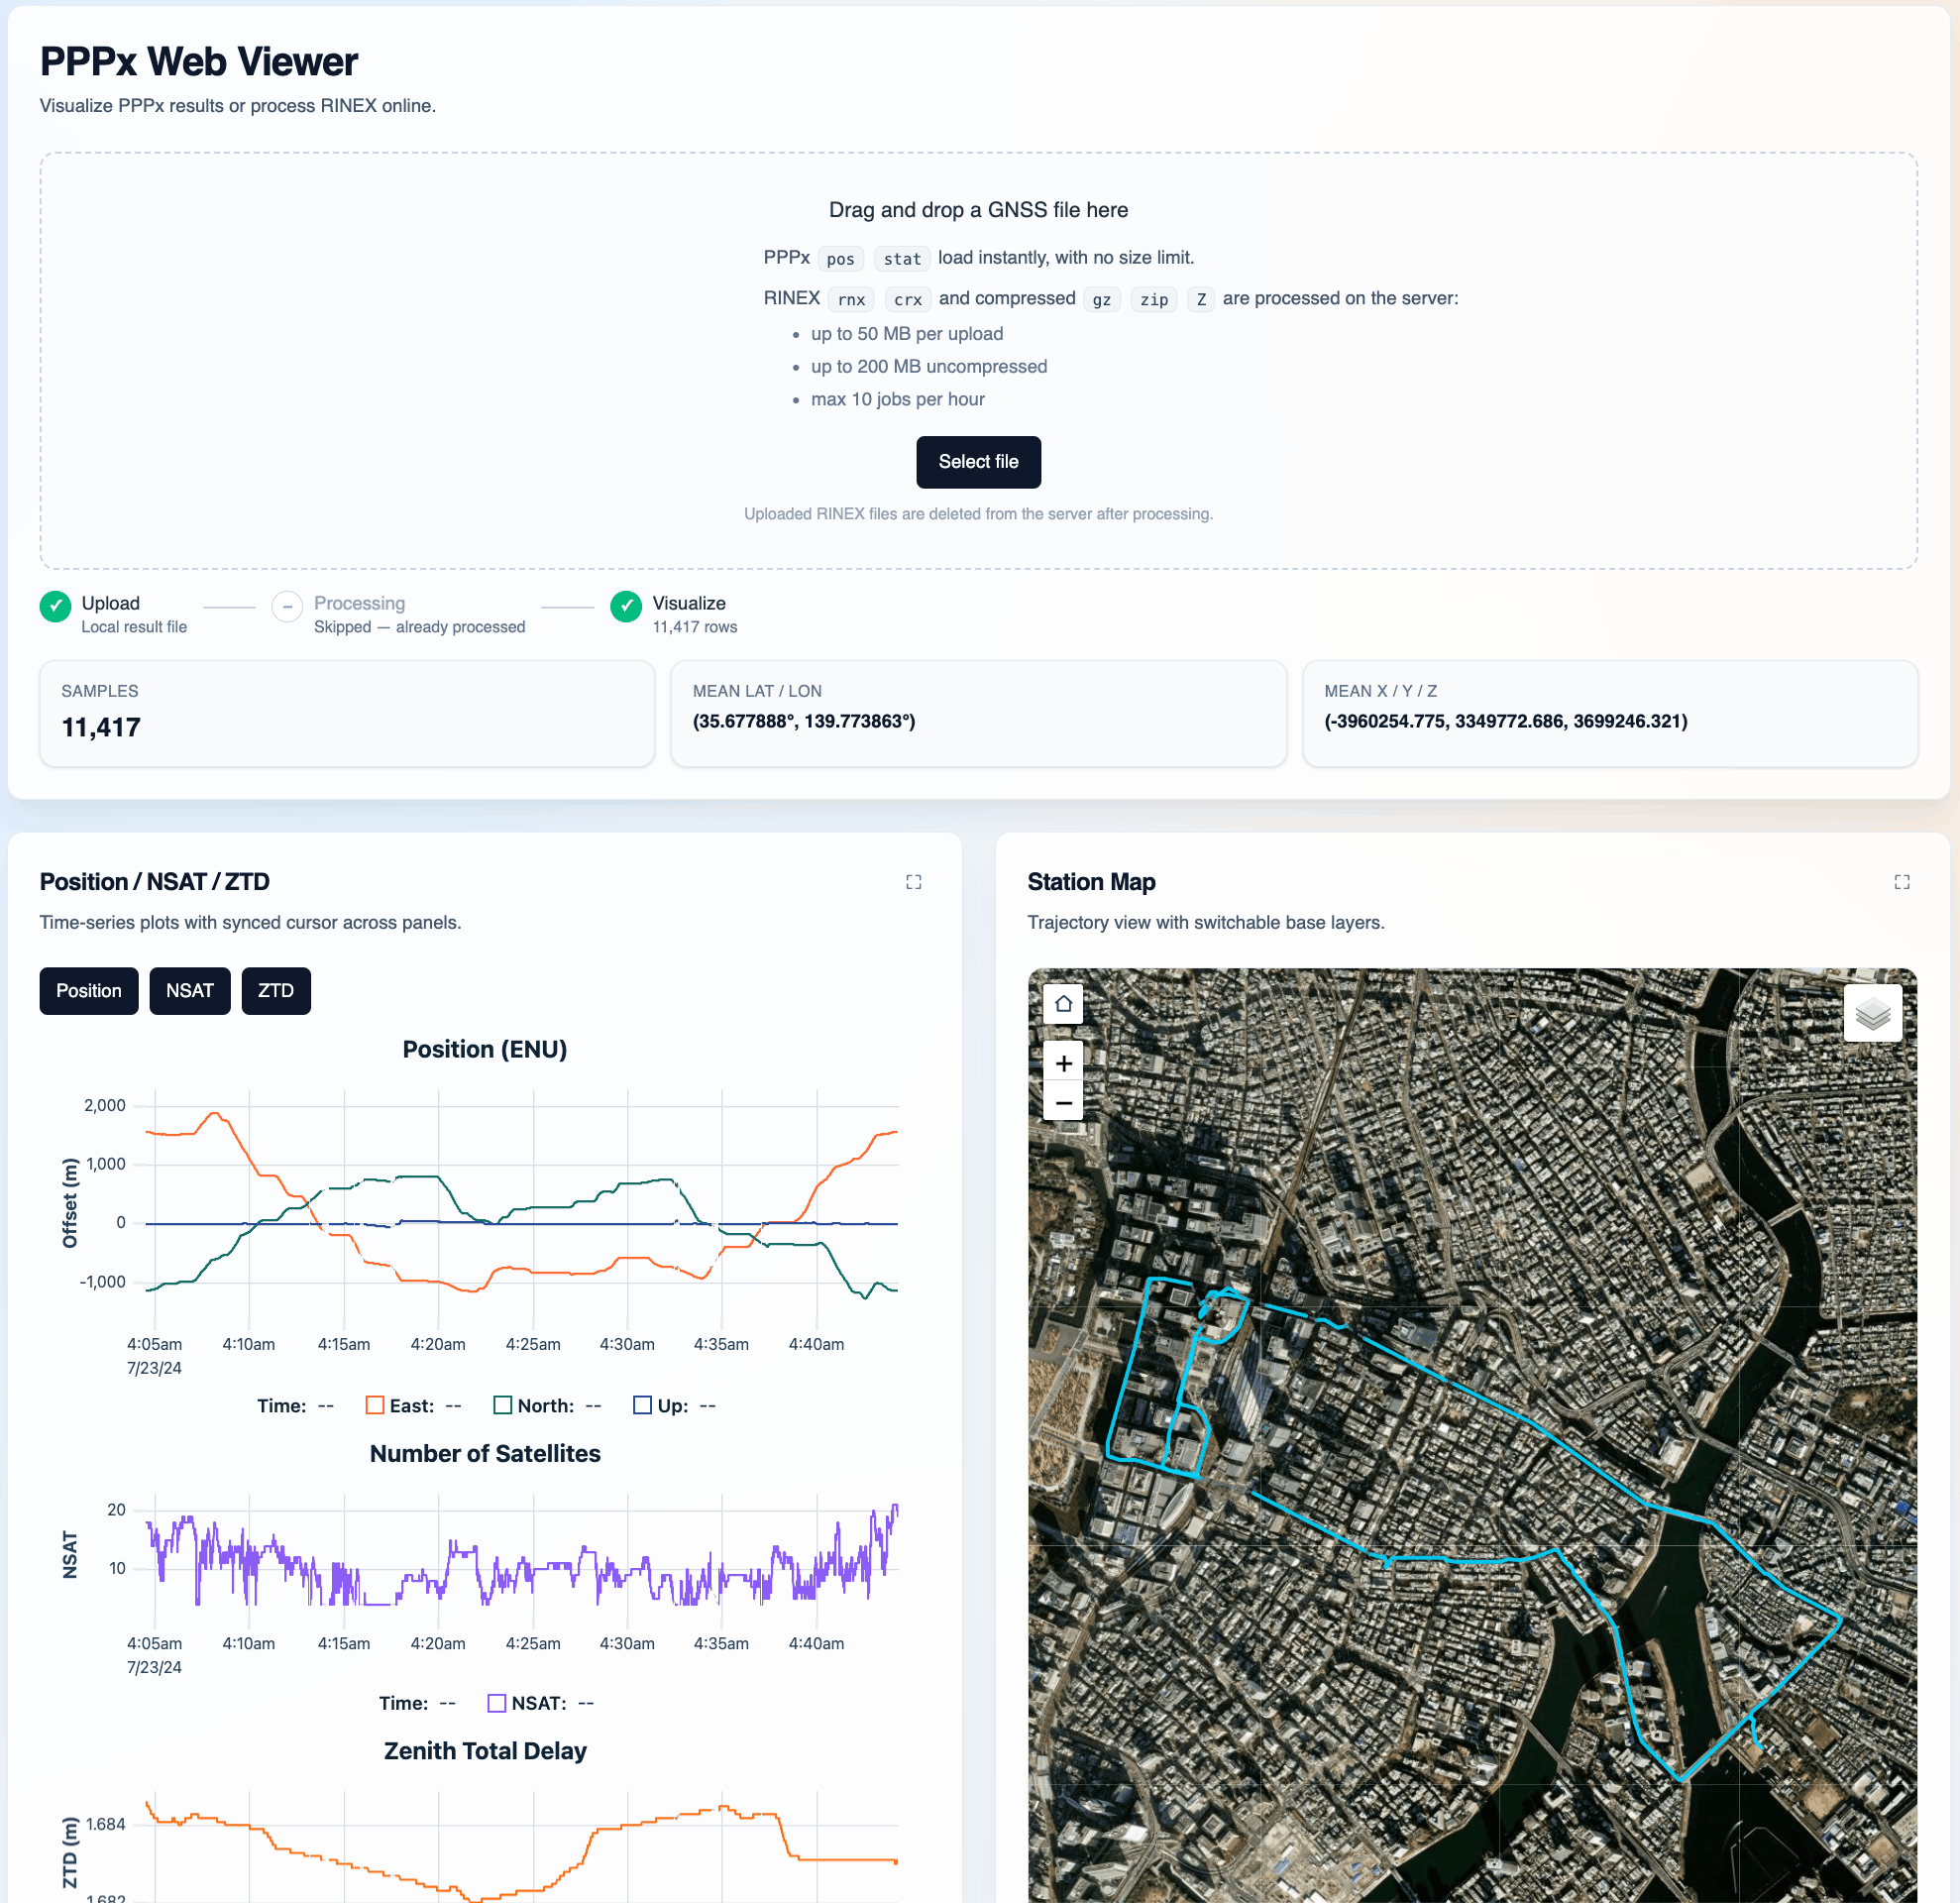
\includegraphics[width=0.7\linewidth]{figs/usage/pppx_web_viewer.png}
    \caption{Visualization of a \pppx{} solution with the PPPx Web Viewer.}
    \label{fig:visualization_web}
    \vspace{-8pt}
\end{figure}



\subsubsection{With Python}
\label{sec:visualization_python}

A Python script named "plot\_ppppos.py" is included in the software package
and is located in the "scripts/" folder.
This script can generate plots of either (1) the positioning time series in the east, north,
and up components (relative to the mean position)
or (2) additional time series of the receiver clock and ZTD estimates.
The general usage of the script is demonstrated with the commands below,
and the corresponding figures are shown in Figure~\ref{fig:visiualization_python}:

\begin{minted}[frame=leftline]{bash}
  # (1) plot position estimates only
  $ ../../scripts/plot_ppppos.py pos_file -s

  # (2) plot position, receiver clock, and ZTD estimates
  $ ../../scripts/plot_ppppos.py pos_file -a

  # Options:
  # -a  Plot position, receiver clock, and ZTD estimates
  # -i  Interactive mode
  # -s  Fixed scale for the y-axis; otherwise, the scale is set automatically
\end{minted}

\begin{figure}
\centering
\begin{subfigure}{.35\paperwidth}
  \centering
  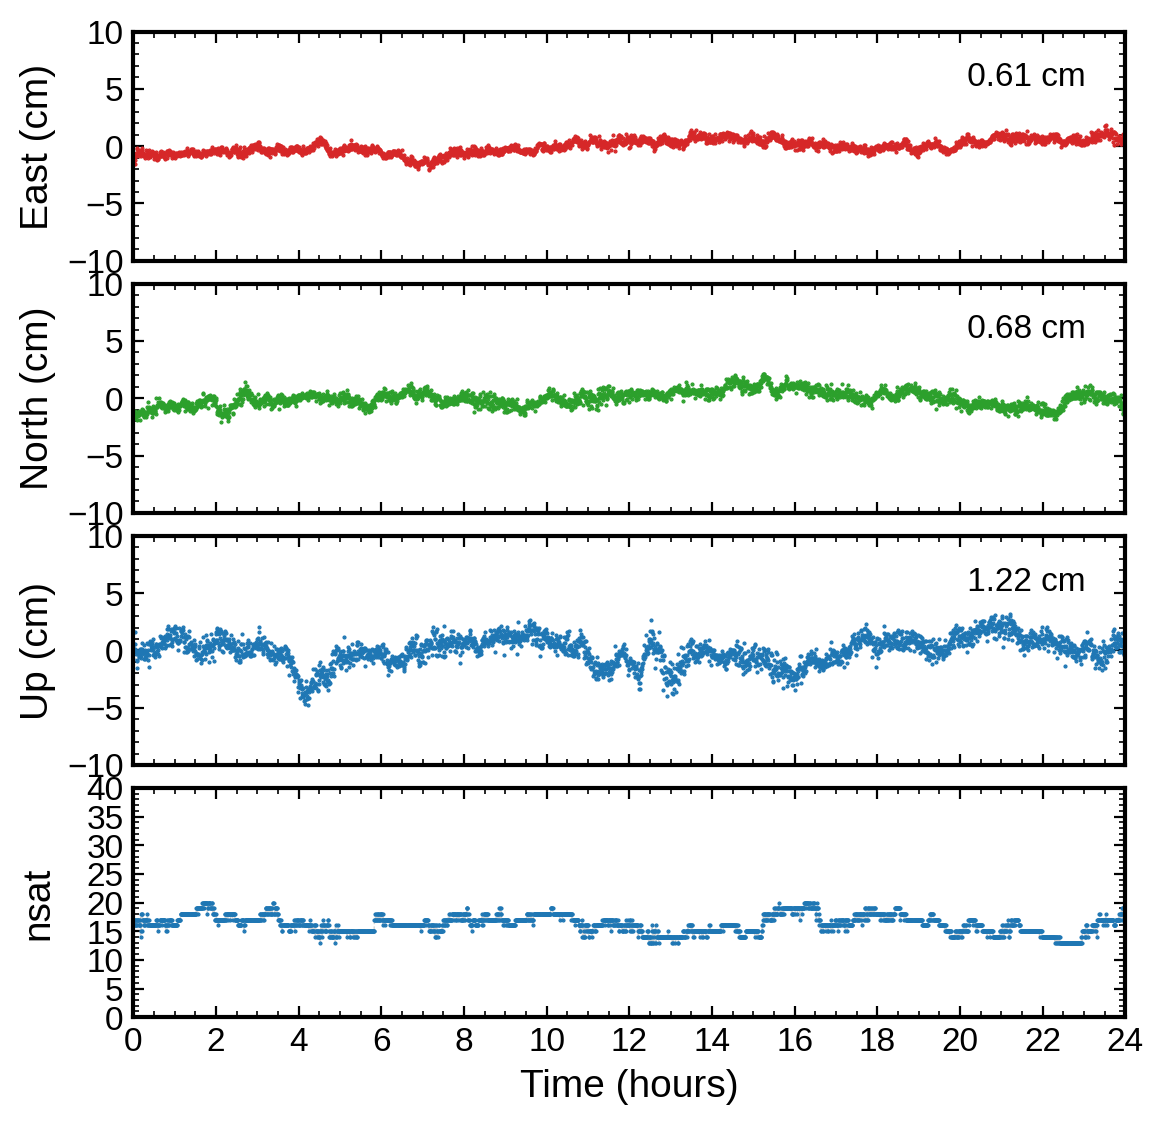
\includegraphics[width=1\linewidth]{figs/examples/ppp_fgo.png}
  \caption{Plotted with option "-s"}
  \label{fig:visualization_python_-s}
\end{subfigure}%
\begin{subfigure}{.35\paperwidth}
  \centering
  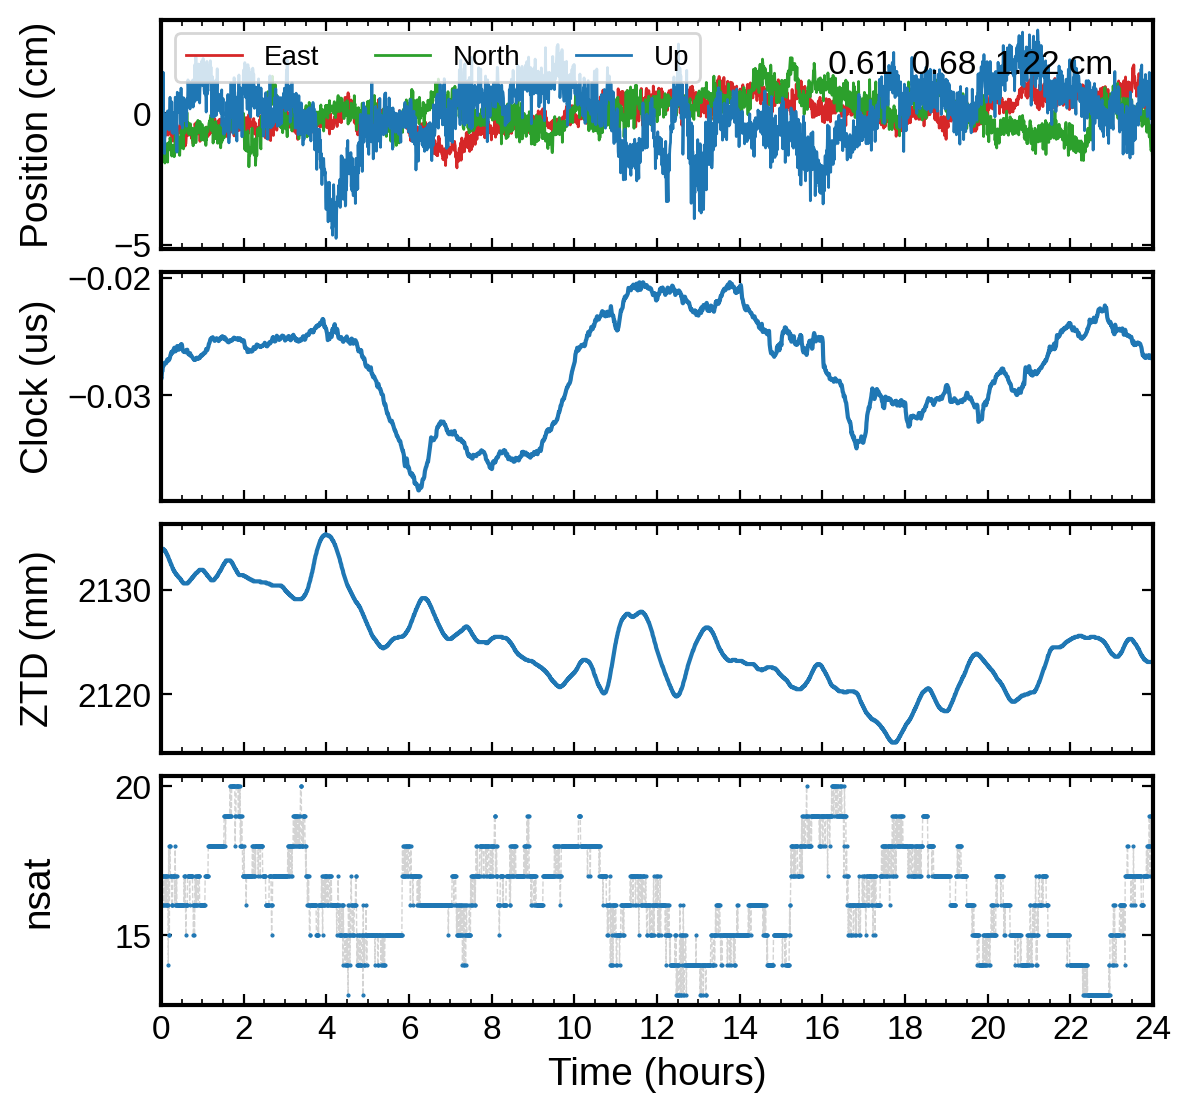
\includegraphics[width=1\linewidth]{figs/usage/python_all.png}
  \caption{Plotted with option "-a"}
  \label{fig:visualization_python_-a}
\end{subfigure}
\caption{Visualization of an FGO-based PPP solution with the Python script.}
\label{fig:visiualization_python}
\end{figure}



\subsubsection{With RTKLIB}
\label{sec:visualization_rtklib}

The \href{https://github.com/tomojitakasu/RTKLIB_bin/tree/rtklib_2.4.3}{RTKLIB} software is
recommended for a richer interactive view of the various plots
and for visualizing post-fit residuals.
One limitation is that the author of RTKLIB provides executables only for Windows;
Linux users must compile the GUI applications themselves using the Qt library.

Using RTKLIB for visualization is straightforward:

\begin{enumerate}
    \item Open the application "rtkplot.exe"
    \item Click the menu "File" > "Open Solution-1" > Select the generated stat file
    \item Interactively view the various plots
\end{enumerate}

Figure~\ref{fig:visiualization_rtklib} shows some example visualizations.
A useful tip: you can open two solutions within the same window for easy comparison.

\begin{figure}
\captionsetup[subfigure]{justification=Centering}
    % \vspace*{-1.55in}
    \hspace*{-.45in}
\begin{subfigure}[t]{0.40\paperwidth}
    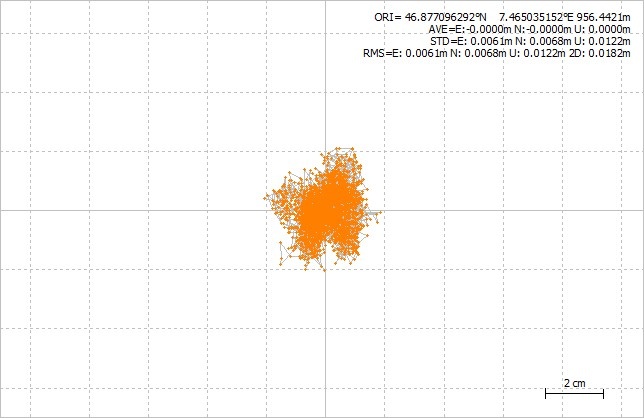
\includegraphics[width=\textwidth]{figs/usage/rtkplot_grd.jpg}
    \caption{Ground track plot.}
\end{subfigure}\hspace{\fill} % maximize horizontal separation
\begin{subfigure}[t]{0.40\paperwidth}
    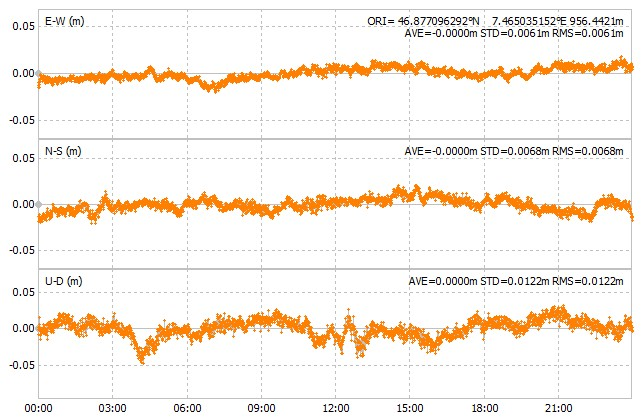
\includegraphics[width=\linewidth]{figs/usage/rtkplot_pos.jpg}
    \caption{Positioning time-series plot.}
\end{subfigure}

% \bigskip % more vertical separation
    \hspace*{-.45in}
\begin{subfigure}[t]{0.40\paperwidth}
    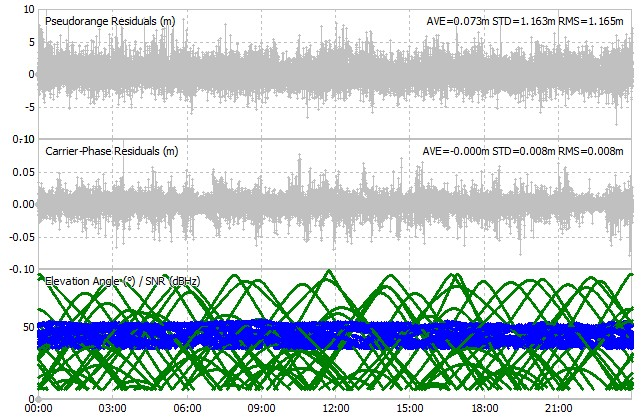
\includegraphics[width=\linewidth]{figs/usage/rtkplot_res_1.jpg}
    \caption{Residual time-series plot.}
\end{subfigure}\hspace{\fill} % maximize horizontal separation
\begin{subfigure}[t]{0.40\paperwidth}
    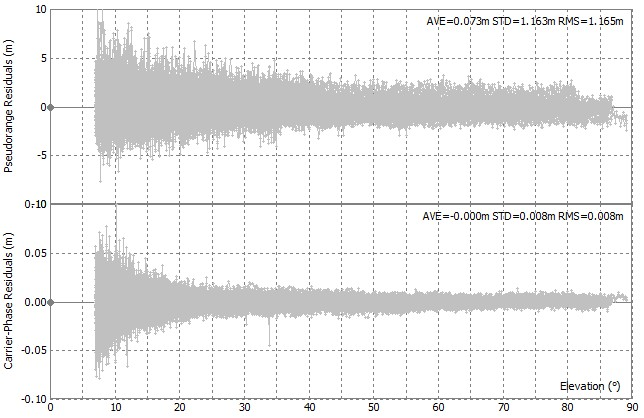
\includegraphics[width=\linewidth]{figs/usage/rtkplot_res_2.jpg}
    \caption{Residual-elevation plot.}
\end{subfigure}
\caption{Visualization of an FGO-based PPP solution with RTKLIB.}
\label{fig:visiualization_rtklib}
\end{figure}

\section{Examples}

This section provides examples of using \pppx{} for various types of data processing.
The corresponding folder is `example/pppx/'.
Specifically, two RINEX files and some products are provided in "example/pppx/rinex/"
and "example/pppx/products/", respectively.
Basic information on the observation and product files can be found in
Tables~\ref{tab:data_for_example} and \ref{tab:products_for_example}, respectively.
Note that the VMF1 grid product is a file splicing the 00 h, 06 h, 12 h, and 18 h epochs
of the current day with the 00 h epoch of the next day.
By default, GPS and Galileo observations are used in each example,
except for the RTK example, which is GPS-only.

% The observations from stations ZIMM and ZIM2 on 2022-100 are used for demonstration.
% The following products are used for positioning:
 
\begin{table}[!hbt]
    \centering
    \caption{GNSS data used in examples.}
    \label{tab:data_for_example}
    \begin{tabular}{ll}
    \toprule
        Data & Description \\
    \midrule
        ZIM200CHE\_R\_20221000000\_01D\_30S\_MO.rnx & Rover station (GREC) \\
        ZIMM00CHE\_R\_20221000000\_01D\_30S\_MO.rnx & Reference station (G) \\
        ALGO00CAN\_R\_20221000000\_15M\_01S\_MO.rnx & High-rate data \\
    \bottomrule
    \end{tabular}
\end{table}


\begin{table}[!hbt]
    \centering
    \caption{Products used in examples.}
    \label{tab:products_for_example}
    \resizebox{\textwidth}{!}{
    \begin{tabular}{ll}
    \toprule
        Product & Description \\
    \midrule
        BRDC00IGS\_R\_20220010000\_01D\_MN.rnx & Broadcast ephemeris for multi-GNSS \\
        COD0MGXFIN\_20221000000\_01D\_05M\_ORB.SP3  & Precise orbit from CODE \\
        COD0MGXFIN\_20221000000\_01D\_30S\_CLK.CLK  & Precise clock from CODE \\
        COD0MGXFIN\_20221000000\_01D\_15M\_ATT.OBX  & Satellite attitude from CODE \\
        COD0MGXFIN\_20221000000\_01D\_01D\_OSB.BIA  & Satellite bias from CODE \\
        COD0MGXFIN\_20221000000\_03D\_12H\_ERP.ERP  & ERP from CODE \\
        codg1000.22i & GIM from CODE \\
        VMFG\_2022100 & spliced VMF1 grid from TU Vienna \\
    \bottomrule
    \end{tabular}}
\end{table}



\subsection{SPP: Single Point Positioning}

The \pppx{} software supports multi-GNSS SPP, including GPS, GLONASS, Galileo, BeiDou, and QZSS,
with broadcast ephemeris or precise satellite products.
Various tropospheric and ionospheric models are supported.
However, only the kinematic mode is currently supported, with either LSQ or FGO as the solver.
Note that LSQ- and FGO-based SPP are both epoch-wise solutions
(i.e., with no constraints between epochs); the only difference is that FGO uses the Huber loss
function (2 m threshold) to improve robustness.
Here, the LSQ solver is used, as the GNSS data in the examples are from geodetic-grade receivers.

Here, SPP solutions using the IF combination and single-frequency observations are demonstrated.
Both examples use broadcast ephemeris, which is the most common case for SPP users.
Specifically, the GMF model and the IF combination are used to correct tropospheric
and ionospheric delays for the IF solution, while the GMF model and a GIM product are used
for the single-frequency solution.
The other settings are kept at their defaults.
The corresponding configuration files can be found as "example/pppx/00\_spp\_if.ini"
and "example/pppx/01\_spp\_sf.ini", respectively.

% Note that the VMF1 model is used only to demonstrate how to use VMF1 grid, and GMF model should be sufficient for SPP. 

% 00\_spp\_if.ini
% \begin{minted}[frame=leftline]{ini}
% [model]
% trop = GMF
% iono = IF

% [product]
% src = brdc
% nav = BRDC_IGS_
% \end{minted}


The positioning results are shown in Figure~\ref{fig:example_spp}.
The single-frequency solution is better than the IF solution.
This is because the IF combination amplifies pseudorange noise by about a factor of three,
while the ionospheric delays can be well corrected with the GIM product for station ZIM2,
which is located at mid-latitude.

\begin{figure}
\centering
\begin{subfigure}{.35\paperwidth}
  \centering
  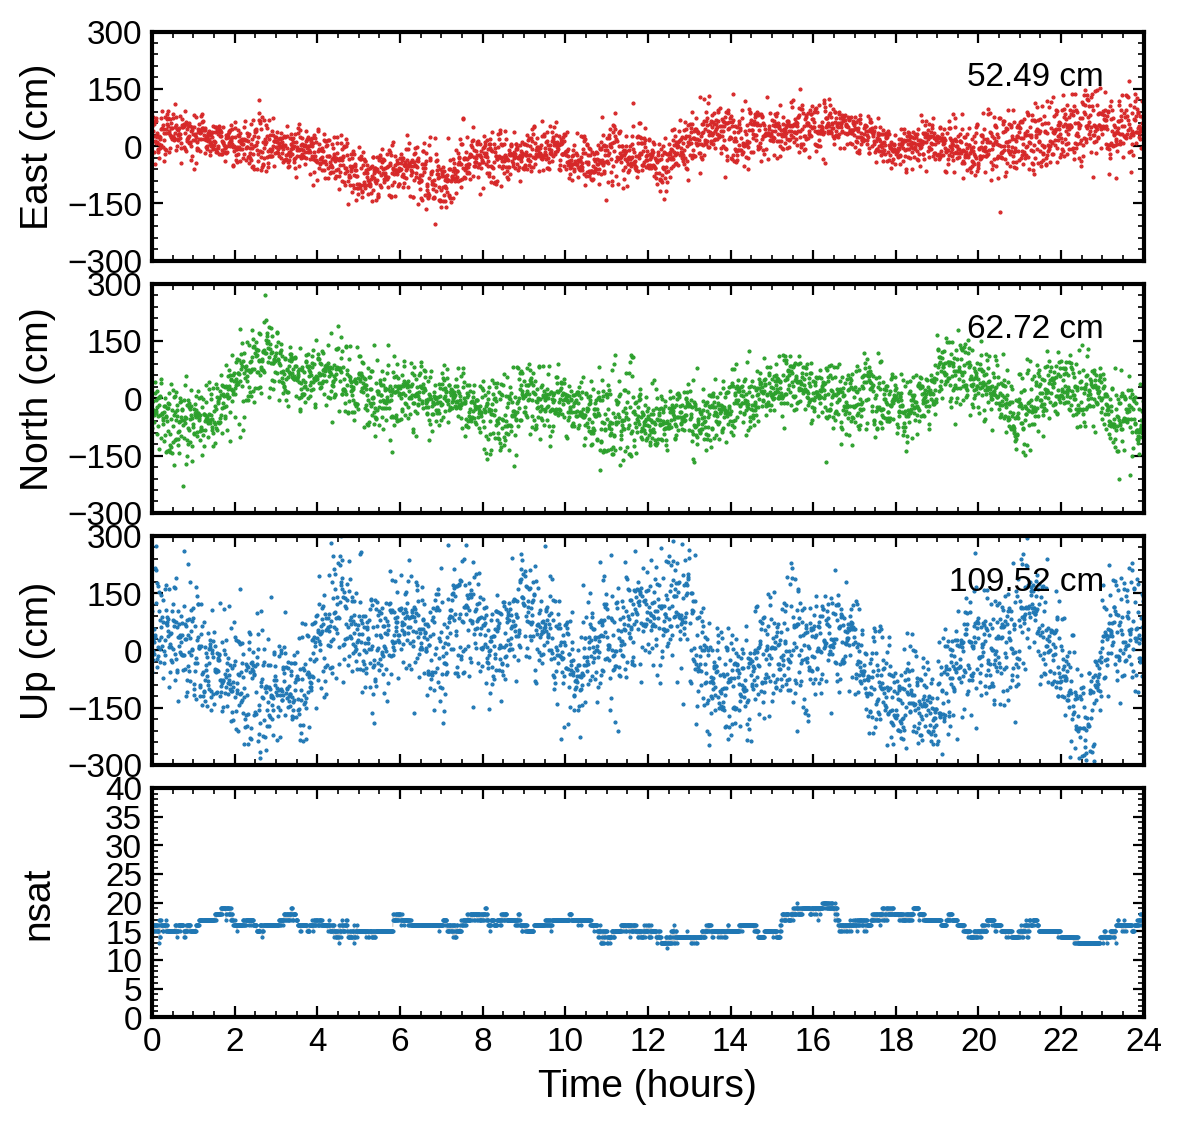
\includegraphics[width=1\linewidth]{figs/examples/spp_if.png}
  \caption{IF solution}
  \label{fig:example_spp_if}
\end{subfigure}%
\begin{subfigure}{.35\paperwidth}
  \centering
  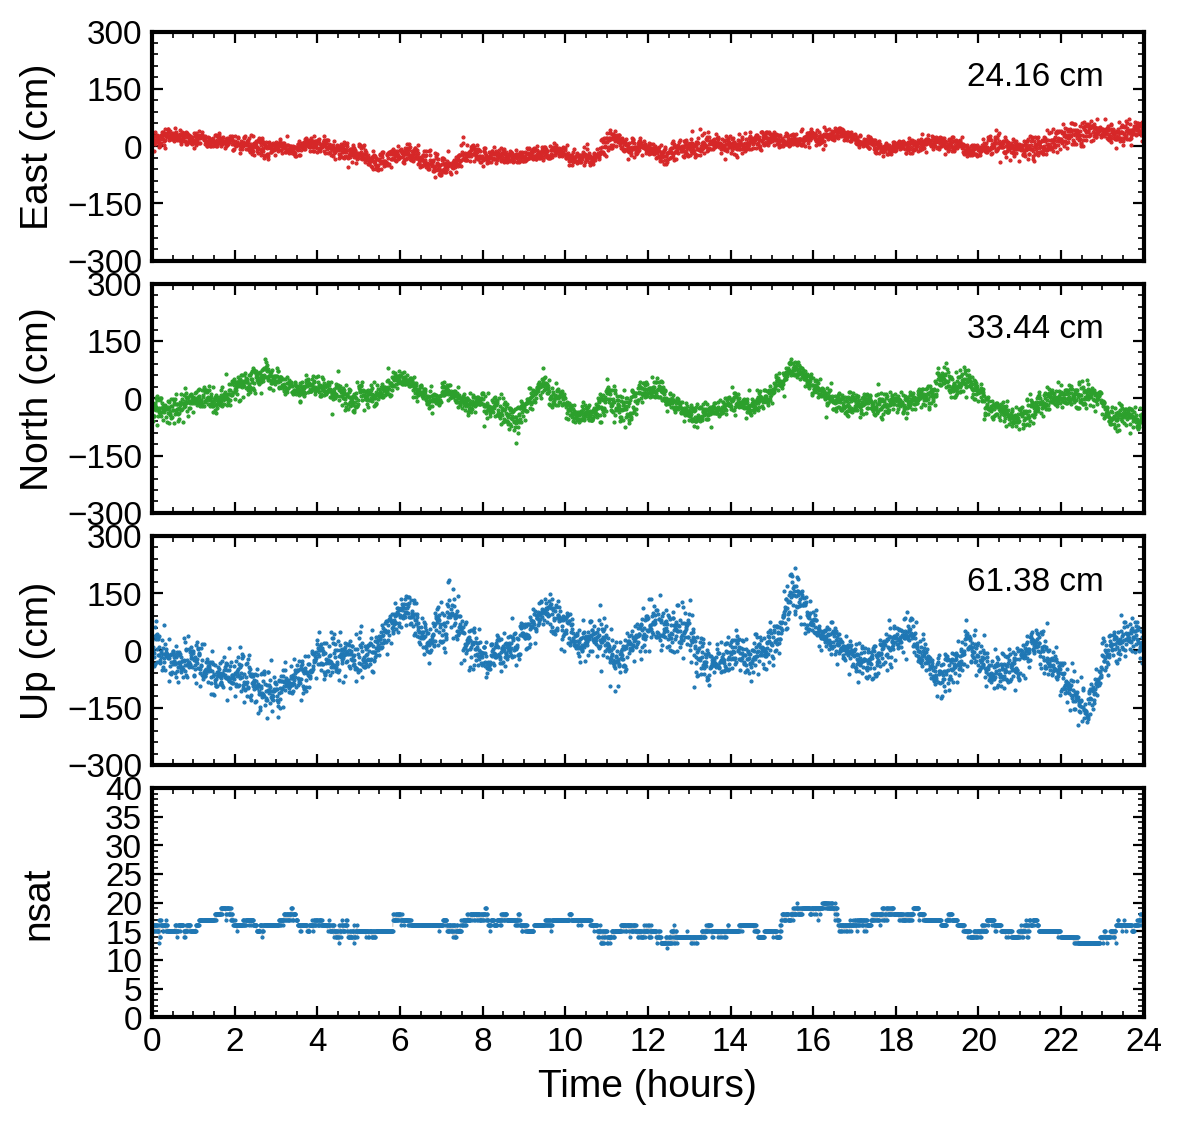
\includegraphics[width=1\linewidth]{figs/examples/spp_sf.png}
  \caption{SF solution}
  \label{fig:example_spp_sf}
\end{subfigure}
% \vspace{-2\baselineskip}
\caption{Positioning results of SPP solutions.}
\label{fig:example_spp}
\end{figure}



\subsection{PPP: Precise Point Positioning}

Here, PPP solutions are demonstrated with the Kalman filter or FGO as the solver.
The corresponding configuration files can be found as "example/pppx/02\_ppp\_ekf.ini"
and "example/pppx/03\_ppp\_fgo.ini", respectively.
The Kalman-filter-based solution simulates the real-time scenario
and outputs a forward-only solution.
The FGO-based solution is dedicated to post-processing and outputs a batch solution,
i.e., one without a convergence period.
In addition, FGO uses the Huber loss function to improve robustness,
with thresholds of 2 m and 0.02 m for pseudorange and carrier phase observations, respectively.

% \begin{enumerate}
%     \item PPP with EKF
%     \item PPP with FGO
%     \item PPP with brdc
% \end{enumerate}

The positioning results are shown in Figure~\ref{fig:example_ppp}.
There is no convergence period for the FGO-based solution,
whereas the EKF solution takes approximately 15 min to converge.
This is because FGO uses all the GNSS observations to form a single large LSQ problem
and solves all the parameters jointly, whereas EKF solves the parameters epoch by epoch.

\begin{figure}
\centering
\begin{subfigure}{.35\paperwidth}
  \centering
  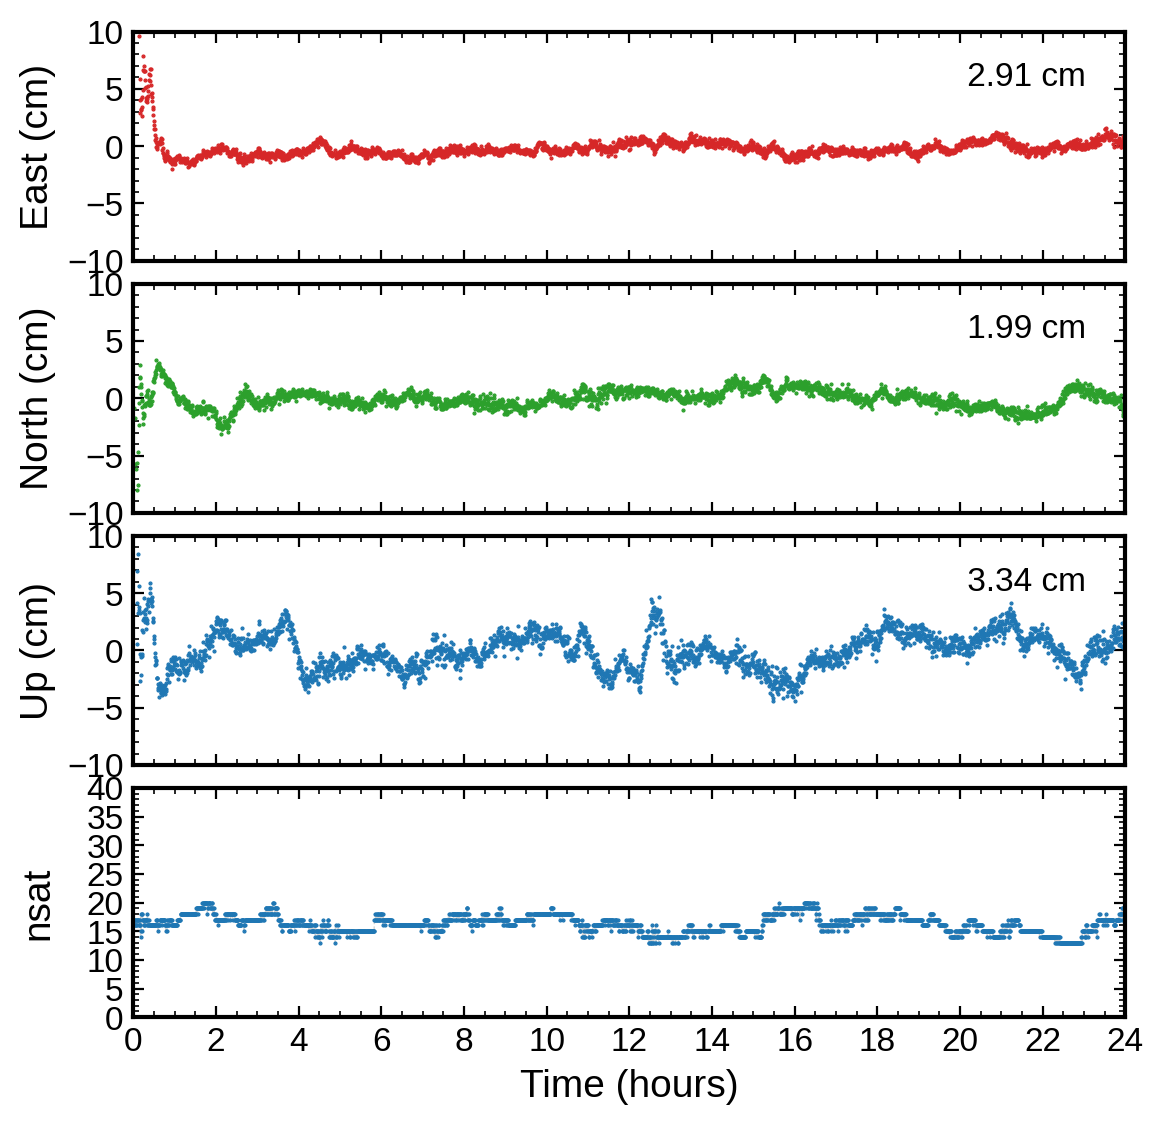
\includegraphics[width=1\linewidth]{figs/examples/ppp_ekf.png}
  \caption{EKF solution}
  \label{fig:example_ppp_ekf}
\end{subfigure}%
\begin{subfigure}{.35\paperwidth}
  \centering
  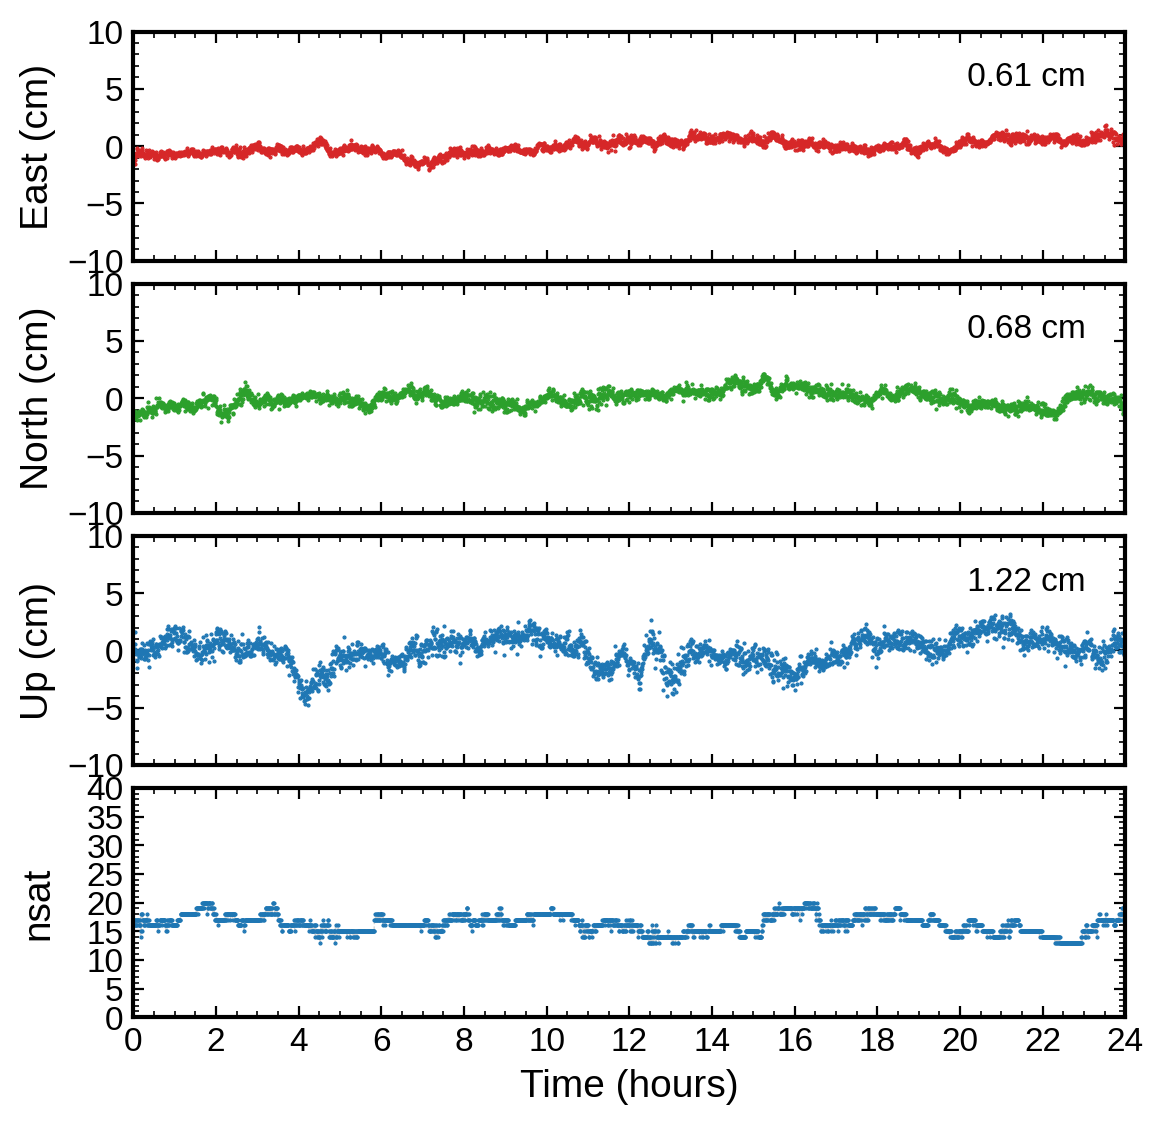
\includegraphics[width=1\linewidth]{figs/examples/ppp_fgo.png}
  \caption{FGO solution}
  \label{fig:example_ppp_fgo}
\end{subfigure}
% \vspace{-2\baselineskip}
\caption{Positioning results of PPP solutions.}
\label{fig:example_ppp}
\end{figure}



\subsection{RTK: Real-Time Kinematic}

The \pppx{} software only supports short baseline solutions.
Thus, "[model] trop" and "[model] iono" are always set to "none".
Both EKF and FGO are supported as solvers for RTK.
As before, the EKF solution simulates the real-time scenario and outputs a forward-only solution,
while the FGO solution is dedicated to post-processing
and outputs a batch solution without a convergence period.
The same Huber loss function as in PPP is adopted for FGO-based RTK processing.
Here, we show the RTK solution computed with EKF as an example.
The corresponding configuration file can be found as "example/pppx/06\_rtk.ini".

\begin{figure}[!hbt]
    \centering
    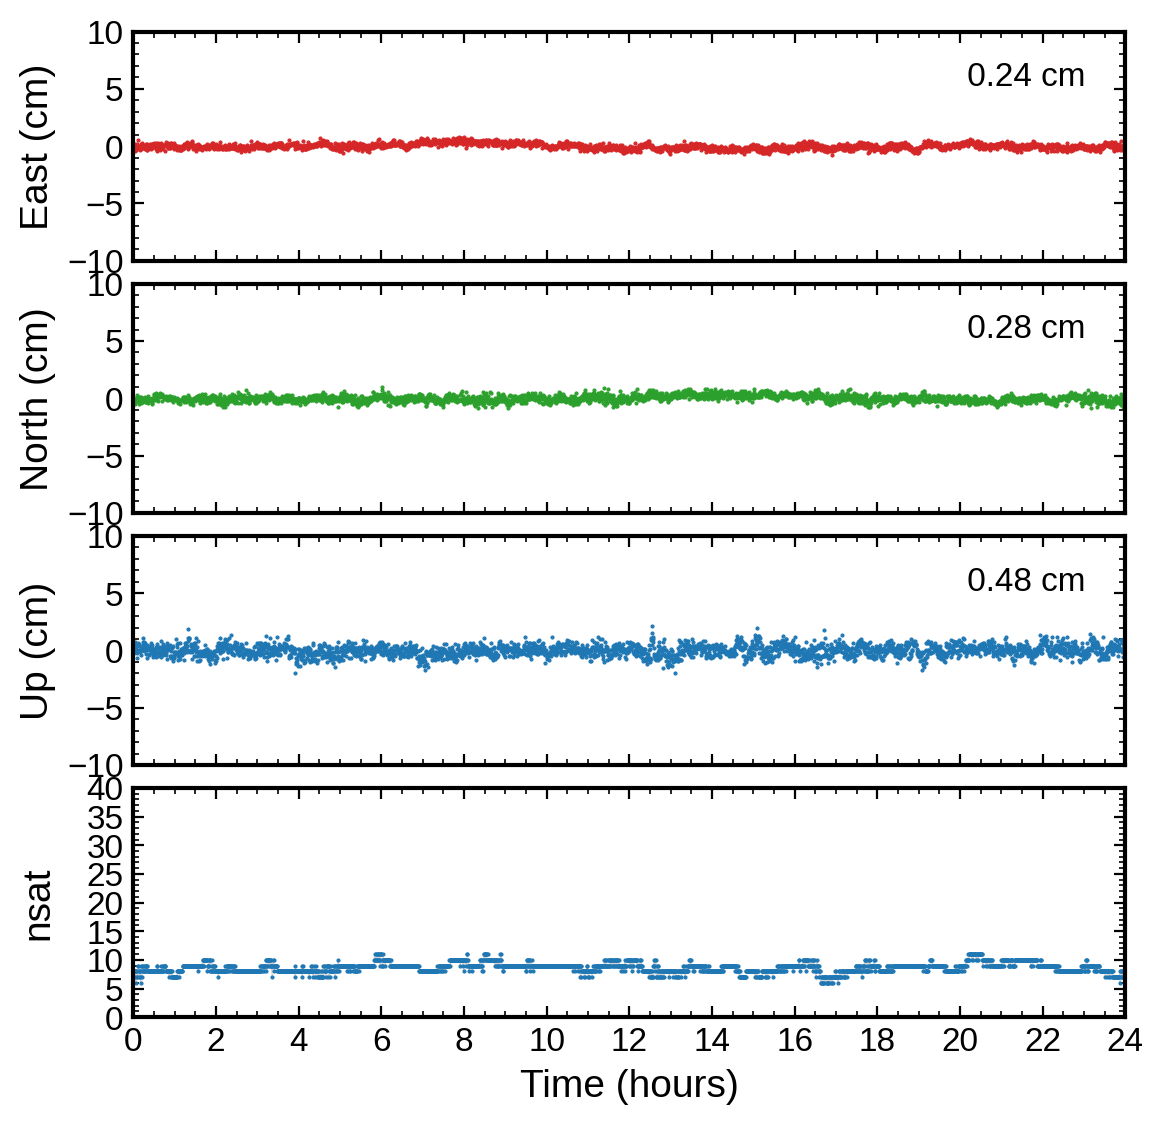
\includegraphics[width=.5\linewidth]{figs/examples/rtk.png}
    \caption{Positioning results of a short baseline solution between ZIM2 and ZIMM.}
    \label{fig:example_rtk}
    \vspace{-8pt}
\end{figure}

The positioning result is shown in Figure~\ref{fig:example_rtk}.
The precision is 0.24 cm, 0.28 cm, and 0.48 cm for the east, north, and up components, respectively.
These are typical precision values for short baseline solutions with resolved ambiguities.



\subsection{TDP: Time-Differenced Positioning}

TDP is useful for earthquake studies because it has no convergence time
and achieves high precision over a short time span.
Ambiguities are eliminated by time-differencing,
and the station displacements between adjacent epochs are estimated.
The displacements are then accumulated onto the initial station position,
and the absolute position for each epoch is written to the pos file.

An example is provided as "07\_tdp", where the 1-Hz GNSS data collected at the ALGO station
are processed with TDP.
Specifically, precise satellite products are used instead of broadcast ephemeris.
In this way, the drift in the positioning time series caused by error accumulation
becomes much smaller.
As ALGO is a static station, the ground truth displacement is zero.
The TDP positioning precisions over 15~min are 0.28~cm, 0.59~cm, and 0.93~cm
in the east, north, and up components, respectively.

\begin{figure}
    \centering
    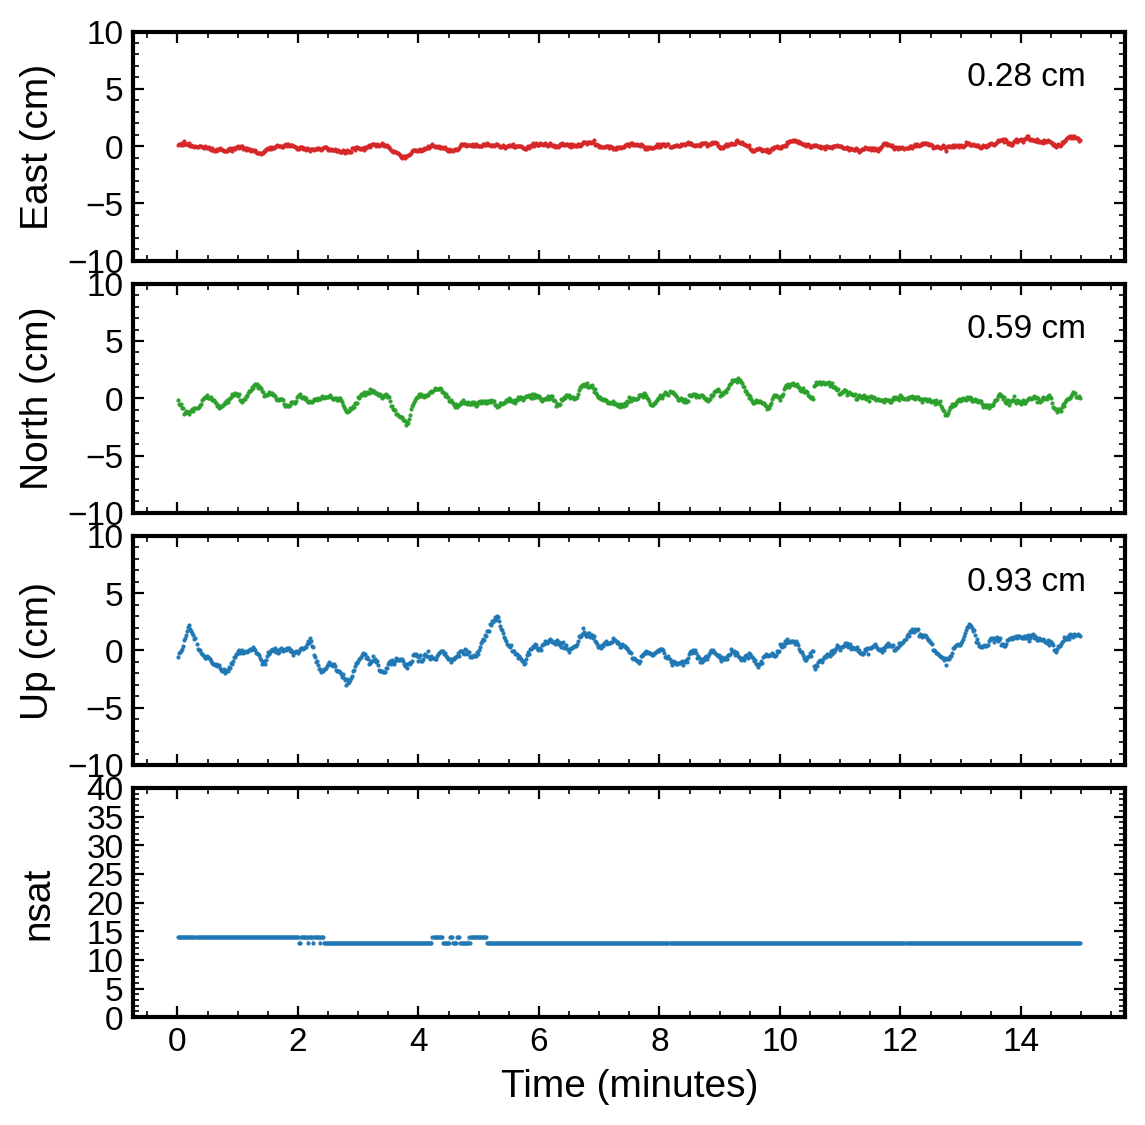
\includegraphics[width=.5\linewidth]{figs/examples/tdp.png}
    \caption{TDP positioning results for the ALGO station.}
    \label{fig:example_tdp}
    \vspace{-8pt}
\end{figure}

\include{src/05_troubleshooting}

\section{FAQs}

Text

% \doclink{https://github.com/tomojitakasu/RTKLIB}{RTKLIB}

\appendix
\section{File Download}

\subsection{Download GNSS observations}

\begin{enumerate}
    \item CDDIS: \url{https://cddis.nasa.gov/archive/gnss/data}
    \item EPN: \url{ftp://ftp.epncb.oma.be/pub/obs}
    \item PBO: \url{https://data.unavco.org/archive/gnss/}
    \item GA: \url{https://data.gnss.ga.gov.au/docs/home/gnss-data.html}
    \item Curtin: \url{http://saegnss2.curtin.edu/ldc}
    \item Hongkong: \url{https://rinex.geodetic.gov.hk}
    % \item NGS: \url{https://noaa-cors-pds.s3.amazonaws.com/rinex}
\end{enumerate}



\subsection{Download IGS Products}

The following HTTP sites are available for downloading GNSS products:
\begin{enumerate}
    \item CDDIS: \url{https://cddis.nasa.gov/archive/gnss/}
    \item CODE: \url{http://ftp.aiub.unibe.ch/CODE_MGEX/CODE/}
    \item ESA: \url{http://navigation-office.esa.int/products/gnss-products/}
    \item CNES: \url{http://www.ppp-wizard.net/daily.html}
\end{enumerate}


FTP sites:
\begin{enumerate}
    \item CDDIS: \url{ftps://gdc.cddis.eosdis.nasa.gov/gnss/}
    \item CODE: \url{ftp://ftp.aiub.unibe.ch/CODE_MGEX/CODE/}
    \item WHU: \url{ftp://igs.gnsswhu.cn/pub/}
    \item IGN: \url{ftp://igs.ign.fr/pub/igs}
\end{enumerate}

Other products:
\begin{enumerate}
    \item VMF1: \url{http://vmf.geo.tuwien.ac.at/trop_products/GRID/2.5x2/VMF1/VMF1_OP/}
\end{enumerate}



\subsection{Download Table Files}
\label{app:table}

\paragraph{Ocean tide loading} \mbox{} \newline
% \href{http://holt.oso.chalmers.se/loading/index-aside-2404271219.html}{Old portal}

Old portal: \url{http://holt.oso.chalmers.se/loading/index-aside-2404271219.html}

New portal: \url{https://barre.oso.chalmers.se/loading/l.php}

Here, we use the old portal to download oceanload coefficients.

\begin{enumerate}
    \item Ocean tide model -> select \textbf{"FES2004"}
    \item Keep other options as default values
    \item Enter the station list: either XYZ or BLH
    \item Enter an email address and click \textbf{"Submit"}
\end{enumerate}

The required oceanload coefficients will be sent to you by email, and then you need to append the coefficients to the table file "table/oceanload".


\paragraph{ANTEX} \mbox{} \newline
\url{https://files.igs.org/pub/station/general}



% \paragraph{Reference} \mbox{} \newline
% \url{https://github.com/zhouforme0318/GAMPII-GOOD/tree/master/doc}

% \listoflistings

\end{document}
